\section{FITS format}
All images acquired from AGO70 are in the format of Flexible Image Transform System (FITS) files. It's an open standard digital format, which is very common for storing astronomical data. This data format will be used within this thesis. The structure of the FITS file is made up of two parts: header and data block \cite{fits}.

A header is a readable data structure that contains multiple keyword/value pairs. It is used for storing image metadata such as size, coordinates, and origin. With astronomical data, the header is very useful in providing photometric and spatial calibration information such as exposure time, readout noise, RADEC coordinates, etc \cite{fits}. An example of the FITS header of the image acquired by AGO70 is shown in the Figure \ref{img:fitsheader}. 

\begin{figure}[h]
    \centering
    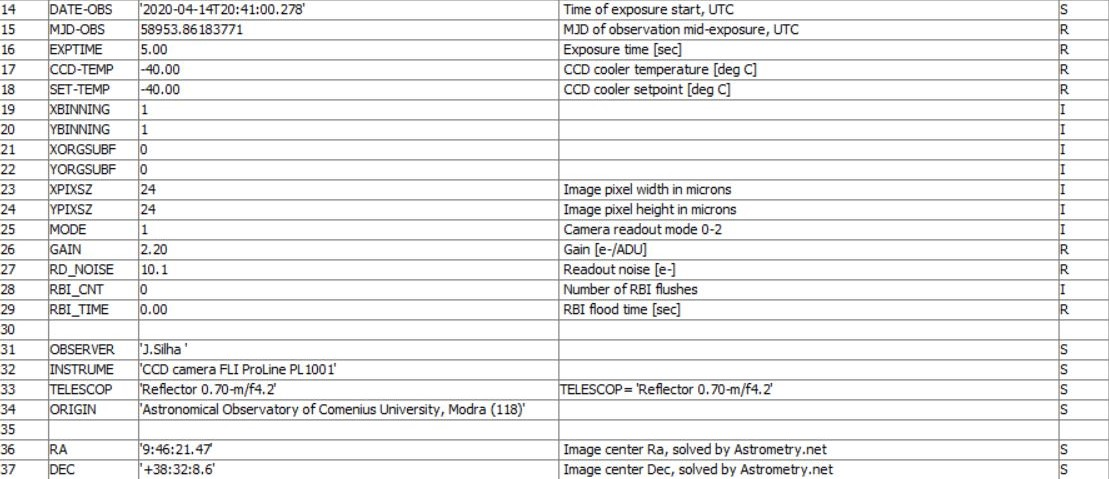
\includegraphics[width=.9\textwidth]{images/fitsheader2.JPG}
    \caption{The FITS header of the image from AGO70.}
    \label{img:fitsheader}
\end{figure}

The data block of the FITS file can store an N-dimensional array of arbitrary size. The data array usually represents an array of image pixel values or tabular data \cite{fits}.